\documentclass[border=5pt]{standalone}
\usepackage{pgfplots}
\pgfplotsset{compat=1.18}
\usepackage{siunitx}
\usepackage{tikz}
\usetikzlibrary{calc}

\definecolor{v2Color}{RGB}{255,80,0}    % Яскраво-помаранчевий (краще видно на білому тлі)
\definecolor{v3Color}{RGB}{0,100,0}     % Темно-зелений (краще контрастує з білим)


\begin{document}
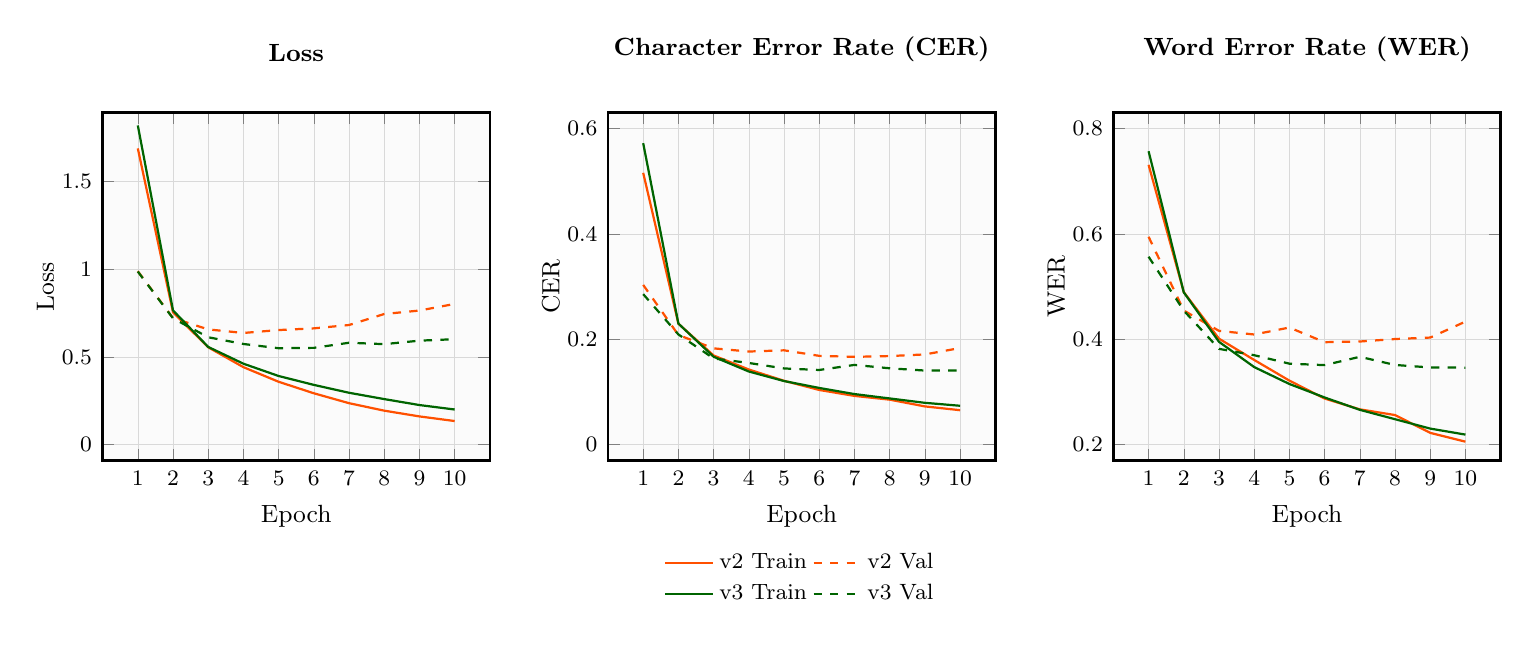
\begin{tikzpicture}[remember picture]

    % Graph 1: Loss
    \begin{axis}[
        name=plot1,
        width=6.5cm,
        height=6cm,
        xlabel={Epoch},
        ylabel={Loss},
        ylabel style={yshift=-0.15cm},
        xmin=0.5, xmax=10.5,
        ymin=0, ymax=1.8,
        xtick={1,2,3,4,5,6,7,8,9,10},
        grid=both,
        grid style={line width=.1pt, draw=gray!10},
        major grid style={line width=.2pt,draw=gray!30},
        title={Loss},
        axis background/.style={fill=gray!3},
        title style={yshift=3mm, font=\small\bfseries},
        label style={font=\small},
        tick label style={font=\footnotesize},
        line width=1pt,
        enlarge x limits=0.05,
        enlarge y limits=0.05,
        every axis plot/.append style={no markers},
        legend to name=commonlegend,
        legend columns=2,
        legend style={draw=none, fill=none, font=\footnotesize}
    ]
        % v2 Train
        \addplot[color=v2Color, thick] coordinates {
            (1, 1.6864) (2, 0.7533) (3, 0.5544) (4, 0.4414) (5, 0.3582)
            (6, 0.2928) (7, 0.2364) (8, 0.1938) (9, 0.1611) (10, 0.1348)
        };
        
        % v2 Validation
        \addplot[color=v2Color, thick, dashed] coordinates {
            (1, 0.9872) (2, 0.7209) (3, 0.6562) (4, 0.6361) (5, 0.6526)
            (6, 0.6623) (7, 0.6813) (8, 0.7440) (9, 0.7637) (10, 0.8013)
        };
        
        % v3 Train
        \addplot[color=v3Color, thick] coordinates {
            (1, 1.8171) (2, 0.7644) (3, 0.5564) (4, 0.4611) (5, 0.3911)
            (6, 0.3405) (7, 0.2957) (8, 0.2597) (9, 0.2258) (10, 0.2004)
        };
        
        % v3 Validation
        \addplot[color=v3Color, thick, dashed] coordinates {
            (1, 0.9856) (2, 0.7193) (3, 0.6116) (4, 0.5733) (5, 0.5492)
            (6, 0.5513) (7, 0.5804) (8, 0.5724) (9, 0.5923) (10, 0.6006)
        };
        
        \legend{v2 Train, v2 Val, v3 Train, v3 Val}
    \end{axis}
    
    % Graph 2: CER, positioned to the right of plot1
    \begin{axis}[
        name=plot2,
        at={($(plot1.east)+(1.5cm,0)$)},
        anchor=west,
        width=6.5cm,
        height=6cm,
        xlabel={Epoch},
        ylabel={CER},
        ylabel style={yshift=-0.15cm},
        xmin=0.5, xmax=10.5,
        ymin=0, ymax=0.6,
        xtick={1,2,3,4,5,6,7,8,9,10},
        grid=both,
        grid style={line width=.1pt, draw=gray!10},
        major grid style={line width=.2pt,draw=gray!30},
        title={Character Error Rate (CER)},
        axis background/.style={fill=gray!3},
        title style={yshift=3mm, font=\small\bfseries},
        label style={font=\small},
        tick label style={font=\footnotesize},
        line width=1pt,
        enlarge x limits=0.05,
        enlarge y limits=0.05,
        every axis plot/.append style={no markers}
    ]
        % v2 Train
        \addplot[color=v2Color, thick] coordinates {
            (1, 0.5158) (2, 0.2296) (3, 0.1693) (4, 0.1427) (5, 0.1213)
            (6, 0.1039) (7, 0.0926) (8, 0.0855) (9, 0.0727) (10, 0.0655)
        };
        
        % v2 Validation
        \addplot[color=v2Color, thick, dashed] coordinates {
            (1, 0.3032) (2, 0.2081) (3, 0.1828) (4, 0.1768) (5, 0.1791)
            (6, 0.1686) (7, 0.1667) (8, 0.1682) (9, 0.1713) (10, 0.1834)
        };
        
        % v3 Train
        \addplot[color=v3Color, thick] coordinates {
            (1, 0.5720) (2, 0.2298) (3, 0.1669) (4, 0.1389) (5, 0.1208)
            (6, 0.1077) (7, 0.0961) (8, 0.0878) (9, 0.0795) (10, 0.0739)
        };
        
        % v3 Validation
        \addplot[color=v3Color, thick, dashed] coordinates {
            (1, 0.2857) (2, 0.2092) (3, 0.1637) (4, 0.1551) (5, 0.1447)
            (6, 0.1418) (7, 0.1514) (8, 0.1450) (9, 0.1407) (10, 0.1408)
        };
    \end{axis}
    
    % Graph 3: WER, positioned to the right of plot2
    \begin{axis}[
        name=plot3,
        at={($(plot2.east)+(1.5cm,0)$)},
        anchor=west,
        width=6.5cm,
        height=6cm,
        xlabel={Epoch},
        ylabel={WER},
        ylabel style={yshift=-0.15cm},
        xmin=0.5, xmax=10.5,
        ymin=0.2, ymax=0.8,
        xtick={1,2,3,4,5,6,7,8,9,10},
        grid=both,
        grid style={line width=.1pt, draw=gray!10},
        major grid style={line width=.2pt,draw=gray!30},
        title={Word Error Rate (WER)},
        axis background/.style={fill=gray!3},
        title style={yshift=3mm, font=\small\bfseries},
        label style={font=\small},
        tick label style={font=\footnotesize},
        line width=1pt,
        enlarge x limits=0.05,
        enlarge y limits=0.05,
        every axis plot/.append style={no markers}
    ]
        % v2 Train
        \addplot[color=v2Color, thick] coordinates {
            (1, 0.7310) (2, 0.4895) (3, 0.4012) (4, 0.3608) (5, 0.3216)
            (6, 0.2876) (7, 0.2671) (8, 0.2563) (9, 0.2225) (10, 0.2058)
        };
        
        % v2 Validation
        \addplot[color=v2Color, thick, dashed] coordinates {
            (1, 0.5945) (2, 0.4546) (3, 0.4160) (4, 0.4091) (5, 0.4223)
            (6, 0.3945) (7, 0.3958) (8, 0.4005) (9, 0.4033) (10, 0.4336)
        };
        
        % v3 Train
        \addplot[color=v3Color, thick] coordinates {
            (1, 0.7569) (2, 0.4890) (3, 0.3952) (4, 0.3473) (5, 0.3152)
            (6, 0.2896) (7, 0.2662) (8, 0.2484) (9, 0.2306) (10, 0.2192)
        };
        
        % v3 Validation
        \addplot[color=v3Color, thick, dashed] coordinates {
            (1, 0.5567) (2, 0.4544) (3, 0.3819) (4, 0.3698) (5, 0.3538)
            (6, 0.3510) (7, 0.3668) (8, 0.3513) (9, 0.3466) (10, 0.3462)
        };
    \end{axis}

    % Positioning the common legend below all graphs
    \node at ($(plot1.south)!0.5!(plot3.south)+(0,-1.5cm)$) {\pgfplotslegendfromname{commonlegend}};
    
\end{tikzpicture}
\end{document}